\section{Heurystyka single swap}

W tym podrozdziale opiszemy heurystykę single swap \cite{Arya2004LocalSH}, która jest przykładem techinki \textit{local search}.
Algorytm przedstawi konstrukcję $(25 + \epsilon)$ aproksymacji dla problemu K-means, która zakłada, że na wejścu dostajemy zbiór kandydatów na centra $C$ oraz zbiór $n$ punktów $P \subset \mathbb{R}^d$.
Autorzy powołują się na pracę \cite{Matousek99onapproximate}, którą zastąpimy pracą \cite{10.1145/1007352.1007400} z uwagi na lepsze gwarancje teoretyczne.
Korzystając z podrozdziału 4.2 w którym przedstawiam \cite{10.1145/1007352.1007400}, obliczamy zbiór $C$.
\\~\\
Heurystyka \textit{single swap} działa poprzez wybranie początkowego zestawu $k$ centrów $S$ z ze zbioru kandydatów na centra $C$, a następnie wielokrotnej
próbie ulepszenia rozwiązania poprzez usunięcie jednego środka $s \in S$ i zastąpienie go innym centerm $s^{'} \in C - S$.
Niech $S^{'} = S - \{s\} \cup \{s^{'}\}$ będzie nowym zbiorem centrów.
Jeżeli $\phi_{S^{'}}(C_{opt}) \leq \phi_{S}(C_{opt})$ to zastępujemy zbiór $S$ zbiorem $S^{'}$, w przeciwnym przypadku $S$ pozostaje bez zmian.
W praktyce taki proces powtarzamy do momentu, kiedy $|\phi_{S^{'}}(C_{opt}) - \phi_{S}(C_{opt})| < \epsilon$.
Formalnie możemy udowodnić, że dla $\epsilon > 0$, po wielomianiwej liczbie wykonań takiej procedury algorytm zakończy swoje działanie.
Autorzy nie dowodzą tego wprosta ale powołują się na pracę \cite{10.1145/380752.380755}.
\\~\\
Dla uproszczenia zakładamy, że algorytm kończy się kiedy pojedyńcza wymiana elementów $s$, $s^{'}$ nie poprawia wyniku.
Taki zbiór centrów nazwiemy \textit{1-stable}.
\begin{definition}
    Zbiór nazywamy \emph{1-stable} jeżeli:
    \begin{equation}
        \Delta(S - \{s\} \cup \{c\}) \leq \Delta(S)
    \end{equation}
    dla dowolnych $s \in S$ oraz $c \in C_{opt}$.
\end{definition}

\noindent
W ramach tego podrozdziału udowodnimy następujące twierdzenie.

\begin{thm}
    Niech $S$ będzie zbiorem $k$ centrów spełniającym własność 1-stable oraz niech $C_{opt}$ będzie optymalnym zbiorem $k$ centrów.
    Wtedy zachodzi następującą nierówność:
    \begin{equation}
        \Delta(S) \leq 25 \Delta(C_{opt})
    \end{equation} 
\end{thm}

\begin{lemma}
    Dla danego skończonego podzbioru $S$ punktów z $\mathbb{R}^d$, niech $c$ będzie centroidem dla $S$. Wtedy dla dowolnego $c^{'} \in \mathbb{R}^d$, $\Delta(S, c^{'}) = \Delta(S, c) + |S|\Delta(c, c^{'})$.
\end{lemma}
\begin{proof}
    Z definicji $\Delta(S, c^{'})$ otrzymujemy:
    \begin{equation}
        \Delta(S, c^{'}) = \sum_{u \in S} \Delta(u, c^{'}) =  \sum_{u \in S} (u - c^{'}) (u - c^{'})
    \end{equation}
    \begin{equation}
         = \sum_{u \in S} ((u - c) + (c - c^{'})) ((u - c) + (c - c^{'}))
    \end{equation}
    \begin{equation}
        = \sum_{u \in S} ((u - c)(u - c)) + 2((u - c)(c - c^{'})) + ((c - c^{'})(c - c^{'}))
    \end{equation}
    \begin{equation}
        = \Delta(S, c) + 2\Big( (c - c^{'}) \sum_{u \in S} (u - c) \Big) + |S|((c - c^{'})(c - c^{'}))
    \end{equation}
    \begin{equation}
        = \Delta(S, c) + |S|\Delta(c,c^{'})
    \end{equation}
    Ostanie przejście korzysta z faktu, że jeżeli $c$ jest centroidem $S$ to zachodzi $\sum_{u \in S} (u - c) = 0$
\end{proof}

%\epsilon
\noindent
Dla każdego optymalnego $c \in C_{opt}$ wyznaczamy $s_{c}$, czyli najbliższe heurestyczne centrum z $S$ dla $c$.
W takim kontekście powiemy, że $c$ jest \textit{schwytane} przez $s_{c}$.
Tutaj warto zaznaczyć, że każde optymalne centrum jest schwytane przez jedno heurystyczne centrum, ale każde heurystyczne centrum może być schwytane przez kilka optymalnych centrów.
Heurystyczne centrum nazwiemy \textit{samotnym} jeżeli nie jest schwytane przez żadne optymalne centrum.

\begin{proof}
    Dowód twierdzenia zaczniemy od zdefniowania podziału $S$ oraz $C_{opt}$ na zbiory $S_{1}, \dots, S_{r}$ oraz $O_{1}, \dots, O_{r}$ dla pewnego $r$, gdzie $|S_{i}| = |O_{i}|$ dla $i = 1, \dots, r$.
    \begin{figure}[H]
        \centering
        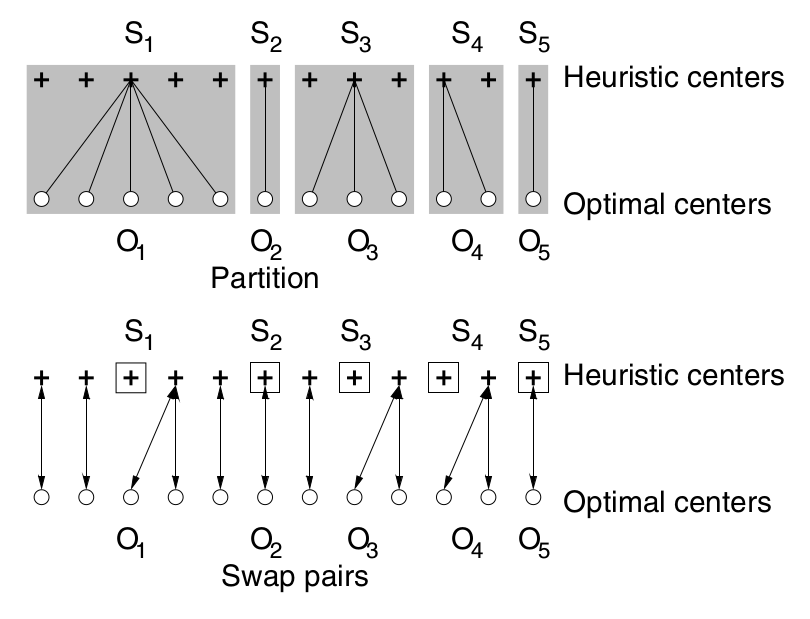
\includegraphics[totalheight=8cm]{swap.png}
        \caption{}
    \end{figure}
    Dla każdego heurystycznego centrum $s_{i}$, które schywało jakąś liczbę $m \geq 1$ optymalnych centr, tworzymy zbior $S_{i}$, który będzie zawierał $s_{i}$ oraz dowolne $m-1$ osamotnionych heurystycznych centr.
    Analogicznie, zbior $O_{i}$ będzie zawierał wszystkie optymalne centra schwytane przez $s_{i}$.
    Rysunek 4.2 obrazuje tak zdefiniowany podział.
    \\~\\
    \noindent
    Następnie będziemy chcieli zdefiniować \textit{swap pary}.
    Dla każdego podziału $|S_{i}| = |O_{i}| = 1$, tworzymy z nich parę.
    Dla każdego podziału, który zawiera więcej schwytanych centr, czyli $|S_{i}|, |O_{i}| \geq 1$, tworzymy pary między osamotnionymi heurystycznymi centrami a optymalnymi centrami.
    Każde optymalne centrum jest związane z jednym heurystycznym oraz każde osamotnione centrum jest przyporządkowane co najwyżej dwóm optymalnym centrom.
    Centra łaczymy dowolnie. 
    Rysunek 4.2 przedstawia przykładowe swap pary.
    \\~\\
    Teraz chcielibyśmy znaleźć ograniczenie górne na zmianię funkcji $\Delta$ po skorzystaniu ze swap pary $(s_{i}, o_{i})$.
    Zaczniemy od obliczenia najbliższych centr z $S - \{s_{i}\} \cup \{o_{i}\}$ dla punktów z $P$.
    Dla punktów $p \in P$, które należą do $N_{O}(o_{i})$ zmiana $\Delta$ będzie następująca:
    \begin{equation}
        \sum_{q \in N_{O}(o_{i})} (\Delta(q, o_{i}) - \Delta(q, s_{q}))
    \end{equation}
    Każde $q \in N_{S}(s_{i}) \setminus N_{O}(o_{i})$ straciło przypisane mu centrum $s_{i}$ zatem punkt $q$ musi otrzymać nowe centrum.
    Niech $o_{q}$ będzie oznaczało najbliższe centrum dla punktu $q$.
    Skoro $q \notin N_{O}(o_{i})$ to $o_{q} \neq o_{i}$, zatem $s_{i}$ nie schwytało $o_{q}$.
    A więc po skorzystaniu ze swap pary, $s_{o_{q}}$, najbliższe heurystyczne centrum dla $o_{q}$ nadal istnieje.
    Zmiana $\Delta$ po wyborze nowych centr jest co najwyżej równa:
    \begin{equation}
        \sum_{q \in N_{S}(s_{i}) \setminus N_{O}(o_{i})} (\Delta(q, s_{o_{q}}) - \Delta(q, s))
    \end{equation}
    Na tym etapie dowodu koniecznie będzie wprowadzenie dwóch lematów.
    
    \begin{lemma}
        Niech $S$ będzie zbiorem $k$ centrów spełniającym własność 1-stable oraz niech $C_{opt}$ będzie optymalnym zbiorem $k$ centrów.
        Wtedy zachodzi następującą nierówność:
        \begin{equation}
            0 \leq \Delta(O) - 3\Delta(S) + 2R
        \end{equation}
        gdzie, $R = \sum_{q \in P} \Delta(q, s_{o_{q}})$.
    \end{lemma}
    \begin{proof}
        Ponieważ $S$ jest 1-stable to:
        \begin{equation}
           0 \leq \Delta(S) -  \Delta(S - \{s_{i}\} \cup \{o_{i}\})
        \end{equation}
        \begin{equation}
            = \sum_{q \in N_{O}(o_{i})} (\Delta(q, o_{i}) - \Delta(q, s_{q})) + \sum_{q \in N_{S}(s_{i}) \setminus N_{O}(o_{i})} (\Delta(q, s_{o_{q}}) - \Delta(q, s))
        \end{equation}
        Aby rozszerzyć sumę na wszystkie możliwe swap pary zauważamy, że dla każdego optymalnego centrum, jest ono swapnięte tylko raz.
        Zatem każdy punkt $q$ kontrybuuje w pierwszej sumie tylko raz.
        Po drugie zaważmy, że różnca w drugiej sumie jest zawsze niezerowa dlatego rozszerzając zakres sumowania mozemy tylko zwiększyć sumaryczny wynik.
        \begin{equation}
            0 \leq \sum_{q \in P} (\Delta(q, o_{q}) - \Delta(q, s_{q})) + \sum_{q \in P} (\Delta(q, s_{o_{q}}) - \Delta(q, s_{q}))
        \end{equation}
        \begin{equation}
            0 \leq \sum_{q \in P} \Delta(q, o_{q}) - 3 \sum_{q \in P} \Delta(q, s_{q}) + 2\sum_{q \in P} \Delta(q, s_{o_{q}})
        \end{equation}
        \begin{equation}
            0 \leq \Delta(C_{opt}) - 3 \Delta(S) + 2R
        \end{equation}
    \end{proof}
    \noindent
    Wcześniej zdefiniowane $R$ nazywamy sumarycznym kosztem przepisania centrów.
    Korzystając z lematu 3 przekształcamy:
    \begin{equation}
        R = \sum_{o \in O} \sum_{q \in N_{O}(o)} \Delta(q, s_{o}) = \sum_{o \in O} \Delta(N_{O}(o), s_{o}) 
    \end{equation}
    \begin{equation}
        = \sum_{o \in O} (\Delta(N_{O}(o), o) + |N_{o}(O)| \Delta(o, s_{o})
    \end{equation}
    \begin{equation}
        = \sum_{o \in O} \sum_{q \in N_{O}(o)} (\Delta(q, o) + \Delta(o, s_{o}))
    \end{equation}
    \begin{equation}
        \leq \sum_{o \in O} \sum_{q \in N_{O}(o)} (\Delta(q, o) + \Delta(o, s_{q}))
    \end{equation}
    \begin{equation}
        = \sum_{q \in P} (\Delta(q, o_{q}) + \Delta(o_{q}, s_{q}))
    \end{equation}
    gdzie ostatnia nierówność bazuje na fakcie, że dla każdego $q \in N_{O}(o)$ mamy $\Delta(o, s_{o}) \leq \Delta(o, s_{q})$.
    Następnie korzystamy z nierówności trójkąta.
    \begin{equation}
        R \leq  \sum_{q \in P} \Delta(q, o_{q}) + \sum_{q \in P} ( d(o_{q}, q) + d(q, s_{q}))^{2}
    \end{equation}
    \begin{equation}
        = \sum_{q \in P} \Delta(q, o_{q}) + \sum_{q \in P} ( d(o_{q}, q)^{2} + 2d(o_{q}, q)d(q, s_{q}) + d(q, s_{q})^{2})
    \end{equation}
    \begin{equation}
        = 2\sum_{q \in P} \Delta(q, o_{q}) + \sum_{q \in P} \Delta(q, s_{q}) + 2\sum_{q \in P} d(o_{q}, q)d(q, s_{q})
    \end{equation}
    \begin{equation}
        = 2\Delta(O) + \Delta(S) + 2\sum_{q \in P} d(o_{q}, q)d(q, s_{q})
    \end{equation}
    \begin{lemma}
        Niech $\langle o_{i} \rangle$ oraz $\langle s_{i} \rangle$ będą ciągami liczb rzeczywistych dla których zachodzi:
        \begin{equation}
            \alpha^2 = \frac{\sum_{i} s_{i}^{2}}{\sum_{i} o_{i}^{2}}
        \end{equation}
        dla pewnego $\alpha > 0$.
        Wtedy:
        \begin{equation}
            \sum_{i=1}^{n} o_{i} s_{i} \leq \frac{1}{\alpha} \sum_{i=1}^{n} s_{i}^{2}
        \end{equation}
    \end{lemma}
    \begin{proof}
        Z nierówności Schwarza:
        \begin{equation}
            \sum_{i=1}^{n} o_{i} s_{i} \leq \Big( \sum_{i=1}^{n} o_{i}^{2} \Big)^{\frac{1}{2}} \Big( \sum_{i=1}^{n} s_{i}^{2} \Big)^{\frac{1}{2}}
        \end{equation}
        \begin{equation}
            = \Big( \frac{1}{\alpha^{2}}\sum_{i=1}^{n} s_{i}^{2} \Big)^{\frac{1}{2}} \Big( \sum_{i=1}^{n} s_{i}^{2} \Big)^{\frac{1}{2}}
        \end{equation}
        \begin{equation}
            = \frac{1}{\alpha} \sum_{i=1}^{n} s_{i}^{2}
        \end{equation}
    \end{proof}
    Niech $o_{i}$ będzie ciągiem $d(q, o_{q})$ oraz niech $s_{i}$ będzie ciągiem $d(q,s_{q})$ dla wszystkich $q \in P$.
    Z tego wynika, że błąd aproksymacji możemy przedstawić jako:
    \begin{equation}
        \alpha^{2} = \frac{\Delta(S)}{\Delta(O)} = \frac{\sum_{q \in P} d(q,s_{q})^{2}}{\sum_{q \in P} d(q,o_{q})^{2}} =\frac{\sum_{i=1}^{n} s_{i}^{2}}{\sum_{i=1}^{n} o_{i}^{2}}
    \end{equation}
    Korzystając z lematu 5:
    \begin{equation}
        R \leq 2\Delta(O) + \Delta(S) + 2\sum_{q \in P} d(o_{q}, q)d(q, s_{q}) 
    \end{equation}
    \begin{equation}
        \leq 2\Delta(O) + \Delta(S) + \frac{2}{\alpha}\sum_{q \in P} d(q, s_{q})^{2} 
    \end{equation}
    \begin{equation}
        = 2\Delta(O) + \Delta(S) + \frac{2}{\alpha}\Delta(S)
    \end{equation}
    \begin{equation}
        = 2\Delta(O) + \Big(1 + \frac{2}{\alpha} \Big)\Delta(S)
    \end{equation}
    Z lematu 4 wiemy, że:
    \begin{equation}
        0 \leq \Delta(O) - 3\Delta(S) + 2R
    \end{equation}
    \begin{equation}
        = \Delta(O) - 3\Delta(S) + 2\Big(2\Delta(O) + \Big(1 + \frac{2}{\alpha} \Big)\Delta(S)\Big)
    \end{equation}
    \begin{equation}
        \leq 5\Delta(O) - \Big(1 - \frac{4}{\alpha} \Big)\Delta(S)
    \end{equation}
    Powyższą nierówności możemy przekształcić do postaci:
    \begin{equation}
        \frac{5}{1-\frac{4}{\alpha}} \geq \frac{\Delta(S)}{\Delta(O)} = \alpha^{2}
    \end{equation}
    \begin{equation}
        5 \geq \alpha^{2} \Big(1 - \frac{4}{\alpha} \Big)
    \end{equation}
    \begin{equation}
        0 \geq (\alpha - 5)(\alpha + 1)
    \end{equation}
    To implikuje, że $\alpha \leq 5$, więc wcześniej zdefiniowany bład aproksymacji możemy ograniczyć $\alpha^{2} \leq 25$, co kończy dowód twierdzenia 4.2.
\end{proof}